\chapter{Repozytorium i system kontroli wersji}

Pliki projektu oraz pliku z dokumentacją, umieszczone zostaly na zdalnym repozytorium kodu pod adresem \href{https://github.com/KamilDudek00/Projekt-programowanie.git}{https://github.com/KamilDudek00/Projekt-programowanie.git}. GitHub to platforma internetowa do hostowania projektów programistycznych, współpracy zespołowej i kontroli wersji przy użyciu systemu kontroli wersji Git. Oferuje narzędzia umożliwiające programistom pracę nad projektami, zarządzanie kodem źródłowym, śledzenie problemów, zarządzanie zadaniem i współpracę z innymi członkami zespołu.\newline 

GitHub jest jednym z najpopularniejszych serwisów hostujących repozytoria Git i jest szeroko używany w społeczności programistycznej do współpracy nad projektami. Z tego miejsca można bezpośrednio pobrać pliki na dysk lub sklonować repozytorium dzięki czemu od razu można zacząć pracę nad kodem i wprowadzać do repozytorium na GitHub.

\begin{figure}[!ht]
	\centering
		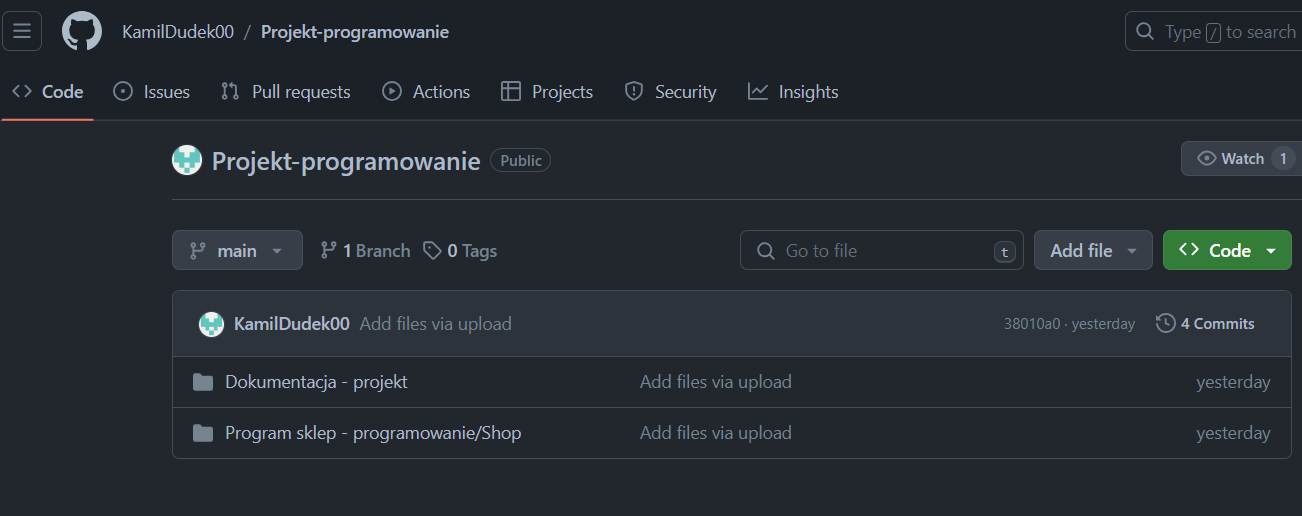
\includegraphics[width=15cm]{screeny/repo.png}
	\caption{\footnotesize Repozytorium z kodem projektu oraz plikami dokumentacji}
	\label{fig:plotend}
\end{figure}